%===================================================================================
\subsection{CU22 Editar tarea}
{
\justify
\color{blue}{\textbf{Objetivo}}
}

%------------------------------------------------------------------
\justify
Permite al Lider de proyecto editar los parametros de la tarea que seleccione.
%------------------------------------------------------------------
{
\justify
\color{blue}{\textbf{Diseño}}
}
%-------------------------------------------------------------------------------
\justify
En la figura \ref{fig:IU22} se muestra la pantalla, en donde permite al Lider de proyecto editar los parametros de la tarea que seleccione.

\begin{figure}[htb]
\centering
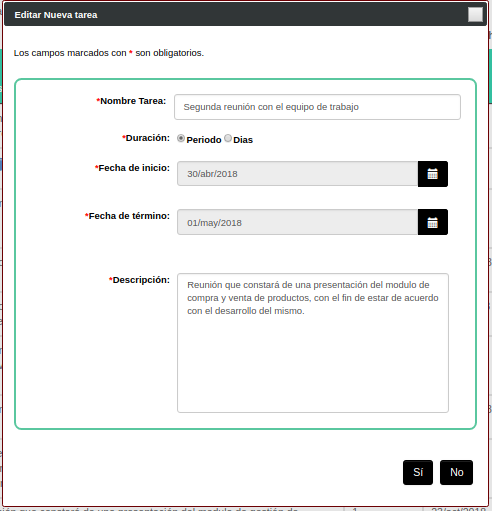
\includegraphics[width=0.8\textwidth]{./images/cu22-editar-tarea.png}
\caption{Editar tarea.} \label{fig:IU22}
\end{figure}